\documentclass[10pt,a4paper]{article}

% --- Page Geometry ---
\usepackage[
    a4paper,
    margin=0.72in,
    top=0.70in,
    bottom=0.70in,
    headheight=13pt,
    headsep=11pt
]{geometry}

% --- Typography & Fonts: Century Schoolbook + Inconsolata + ClearSans ---
\usepackage{fouriernc}
\usepackage[T1]{fontenc}
\usepackage[scaled=0.95]{inconsolata}
\usepackage{ClearSans}
\usepackage{microtype}

% --- Spacing ---
\usepackage{setspace}
\setstretch{1.06}
\usepackage{parskip}
\setlength{\parskip}{2.5pt plus 0.8pt minus 0.5pt}
\setlength{\parindent}{0pt}

% --- Math ---
\usepackage{amssymb}
\usepackage{amsmath, amsthm, mathtools}
\usepackage{bm}
\setlength{\jot}{2pt}

\DeclareSymbolFont{cmssymbols}{OMS}{cmsy}{m}{n}
\DeclareMathSymbol{\forall}{\mathord}{cmssymbols}{"38}
\DeclareMathSymbol{\exists}{\mathord}{cmssymbols}{"39}
\DeclareSymbolFont{cmexsymbols}{OMX}{cmex}{m}{n}
\let\sum\relax
\DeclareMathSymbol{\sum}{\mathop}{cmexsymbols}{"50}

% --- Tables & Graphics ---
\usepackage{booktabs}
\usepackage{array}
\usepackage{tabularx}
\usepackage{multirow}
\usepackage{graphicx}
\graphicspath{{./}{figures/}}
\usepackage{xcolor}
\usepackage[skins,breakable]{tcolorbox}
\renewcommand{\arraystretch}{1.12}

\usepackage{tikz}
\usetikzlibrary{arrows.meta, positioning, calc, shapes.geometric, fit, backgrounds}

% --- Palette ---
\colorlet{docaccent}{blue!60!black}
\definecolor{strings}{HTML}{00999A}
\definecolor{comments}{HTML}{990000}
\definecolor{boxbg}{HTML}{F8FAFC}

\newtcolorbox{promptbox}[1][]{
    enhanced,
    boxrule=0pt,
    frame hidden,
    borderline west={2.5pt}{0pt}{docaccent},
    colback=docaccent!4!white,
    arc=1.5mm,
    left=10pt, right=10pt, top=4.5pt, bottom=4.5pt,
    before skip=4pt, after skip=5pt,
    fontupper=\small\sffamily,
    #1
}

% --- Captions ---
\usepackage{caption}
\DeclareCaptionLabelFormat{customtable}{TABLE #2}
\DeclareCaptionLabelFormat{customfig}{FIGURE #2}
\captionsetup[table]{labelformat=customtable, labelsep=colon, position=above, skip=3pt, font=small, labelfont={bf,sf}, singlelinecheck=false, justification=raggedright}
\captionsetup[figure]{labelformat=customfig, labelsep=colon, position=below, skip=4pt, font=small, labelfont={bf,sf}, singlelinecheck=false, justification=raggedright}

\usepackage{enumitem}
\setlist{itemsep=1.5pt, topsep=2pt, parsep=0.5pt, partopsep=0.5pt}
\setlist[enumerate]{leftmargin=*}
\setlist[itemize]{leftmargin=*}

\usepackage{fancyhdr}
\usepackage{titlesec}
\usepackage{hyperref}
\hypersetup{colorlinks=true, linkcolor=docaccent, urlcolor=docaccent, citecolor=docaccent}

% --- Metadata ---
\newcommand{\CourseCode}{CPE 613}
\newcommand{\CourseName}{Optimization Methods}
\newcommand{\AssignmentNumberText}{TERM PROJECT}
\newcommand{\AssignmentNumberVal}{PHASE I REPORT}
\newcommand{\AssignmentTitle}{Debt Collection Strategy Allocation using Mathematical Programming and Meta-Heuristics}
\newcommand{\SubTitle}{Single-Objective Formulation, Empirical Recovery Estimation, and Scaling Benchmarks}
\newcommand{\AssignmentDate}{25 November 2026}
\newcommand{\StudentOneName}{Yuil Tripathee}
\newcommand{\StudentOneID}{69070701612}
\newcommand{\StudentTwoName}{Sawit Koseeyaumporn}
\newcommand{\StudentTwoID}{69070701621}
\newcommand{\InstructorNames}{Assoc. Prof. Dr. Naruemon Wattanapongsakorn, Dr. Tossaphol Settawatcharawanit}

\pagestyle{fancy}
\fancyhf{}
\fancyhead[L]{\small\sffamily\bfseries\color{docaccent}{\CourseCode} \CourseName}
\fancyhead[R]{\small\sffamily \AssignmentNumberText~\AssignmentNumberVal}
\fancyfoot[C]{\small\sffamily\thepage}
\renewcommand{\headrulewidth}{0.4pt}
\renewcommand{\footrulewidth}{0pt}

\titleformat{\section}
  {\normalfont\large\bfseries\sffamily\color{docaccent}}{\thesection}{1em}{}
  [{\color{docaccent}\titlerule[0.8pt]}]
\titleformat{\subsection}
  {\normalfont\normalsize\bfseries\sffamily\color{docaccent}}{\thesubsection}{1em}{}
\titleformat{\subsubsection}
  {\normalfont\small\bfseries\sffamily\color{docaccent}}{\thesubsubsection}{1em}{}

\titlespacing*{\section}{0pt}{8pt plus 1pt minus 1pt}{3pt plus 1pt minus 1pt}
\titlespacing*{\subsection}{0pt}{5pt plus 1pt minus 1pt}{2pt plus 0.5pt minus 0.5pt}
\titlespacing*{\subsubsection}{0pt}{4pt plus 1pt minus 1pt}{2pt plus 0.5pt minus 0.5pt}

\newcommand{\makeproposalheader}{
  \thispagestyle{plain}
  \begingroup
  \raggedright
  {\normalsize\sffamily\color{gray!70!black}\textbf{\AssignmentNumberText} {\color{docaccent}\textbf{\AssignmentNumberVal}}~(\textbf{\CourseCode: \CourseName})}\\[2pt]
  {\LARGE\sffamily\bfseries\color{docaccent}\AssignmentTitle}\\[2pt]
  {\normalsize\sffamily\color{gray!80!black}\SubTitle}\\[5pt]
  {\color{docaccent}\rule{\textwidth}{1.0pt}}\\[3pt]
  {\small\sffamily
  \textbf{Members:} \StudentOneName~(\texttt{\StudentOneID}), \StudentTwoName~(\texttt{\StudentTwoID}) \hfill \textbf{Date:} \AssignmentDate \\
  \textbf{Instructors:} \InstructorNames \\
  \textbf{Repository:} \texttt{Celesca/cpe613-final-term-optimization-methods}}\\[2pt]
  {\color{docaccent}\rule{\textwidth}{0.4pt}}
  \endgroup
  \vspace{0.2em}
}

\begin{document}

\makeproposalheader

\setcounter{tocdepth}{2}
\begingroup
\small
\setlength{\parskip}{0.4pt}
\tableofcontents
\endgroup
\vspace{0.5em}
{\color{docaccent!40}\hrule height 0.5pt}
\vspace{0.5em}

\section{Project Name}
\textbf{Debt Collection Strategy Allocation using Mathematical Programming and Meta-Heuristics}

\emph{Problem Class:} Multidimensional Multiple-Choice Knapsack Problem with Fixed-Charge Activation (MMKP-FC), formulated as a 0--1 Mixed-Integer Linear Program (MILP).

\section{Student Names and IDs}
\begin{enumerate}
    \item \textbf{\StudentOneName} --- Student ID: \texttt{\StudentOneID}
    \item \textbf{\StudentTwoName} --- Student ID: \texttt{\StudentTwoID}
\end{enumerate}

\section{Project Description and Scope}

\subsection{Problem Statement}
Consumer lenders hold portfolios of delinquent loans across varying delinquency ages and unpaid balances. Every billing cycle, the collections team must assign each delinquent account $i \in \{1,\dots,N\}$ to exactly one recovery channel $k \in \{0,\dots,5\}$:
\begin{enumerate}[label=(\roman*)]
    \item \textbf{No Action / Self-Cure ($k=0$):} Zero direct cost ($\lambda_0 = 0.30$).
    \item \textbf{Digital Reminders ($k=1$):} Automated SMS / LINE OA message ($\text{THB~}25$, $\lambda_1 = 0.55$).
    \item \textbf{In-House Call Center ($k=2$):} Staff call consuming $0.75\text{ h}$ labor ($\text{THB~}350$, baseline $\lambda_2 = 1.00$).
    \item \textbf{Field Collector Visit ($k=3$):} Doorstep visit consuming one visit slot ($\text{THB~}1{,}800$, $\lambda_3 = 1.40$).
    \item \textbf{External Collection Agency ($k=4$):} Third-party handover ($\text{THB~}500 + 25\%$ commission, $\lambda_4 = 1.70$).
    \item \textbf{Legal Action ($k=5$):} External law firm litigation ($\text{THB~}8{,}000 + 2\%$ balance cost, $\lambda_5 = 2.30$), requiring a shared upfront retainer $F = \text{THB~}40{,}000$ and at least $L = 3$ filed cases.
\end{enumerate}
Stronger channels improve recovery probability but face four shared constraints: total collection budget ($B_{\max}$), call-center hours ($H$), field-visit slots ($V$), and a customer-conduct cap ($M$) on combined agency and legal accounts. The single-objective goal of Phase I is to assign strategies to maximize expected net recovery in Thai Baht (THB) net of operational costs, commissions, and legal retainer fees.

\subsection{System Architecture and Phase I Scope}
Figure~\ref{fig:workflow} summarizes the pipeline connecting LendingClub empirical recovery modeling to exact MILP and meta-heuristic solvers.

\begin{figure}[!ht]
\centering
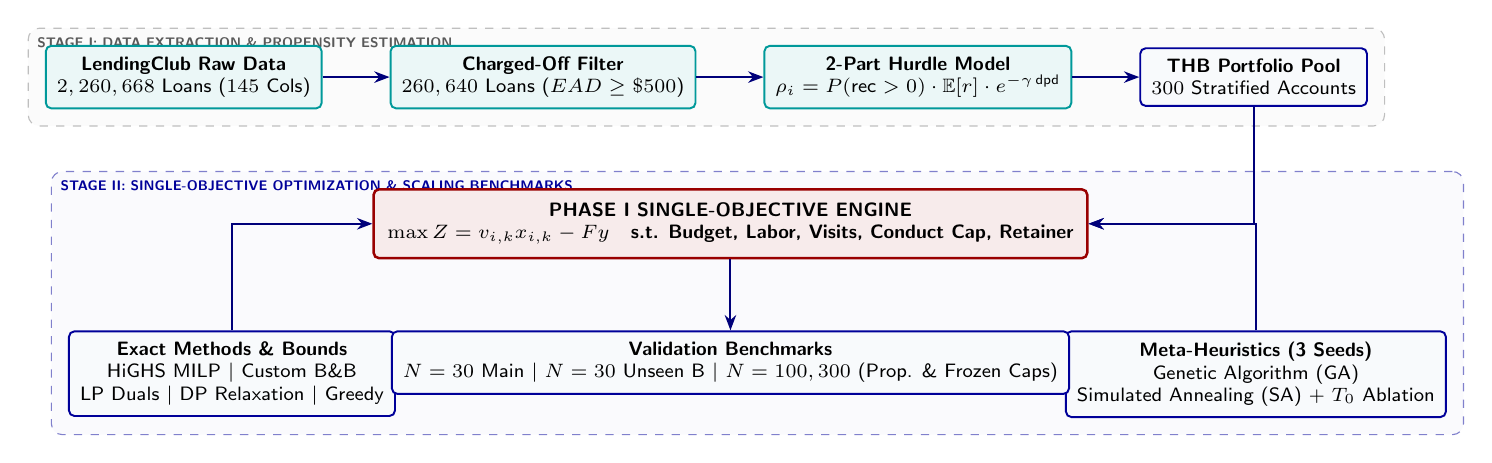
\begin{tikzpicture}[
    node distance=0.8cm and 0.85cm,
    every node/.style={font=\sffamily\scriptsize},
    box/.style={rectangle, draw=docaccent, fill=boxbg, rounded corners=2pt, minimum height=0.62cm, align=center, inner sep=4pt, line width=0.7pt},
    databox/.style={rectangle, draw=strings, fill=strings!8!white, rounded corners=2pt, minimum height=0.62cm, align=center, inner sep=4pt, line width=0.7pt},
    optbox/.style={rectangle, draw=comments, fill=comments!8!white, rounded corners=2pt, minimum height=0.72cm, align=center, inner sep=5pt, line width=0.9pt, font=\sffamily\bfseries\scriptsize},
    arrow/.style={-{Stealth[scale=0.9]}, line width=0.7pt, draw=docaccent!80!black}
]
\node[databox] (raw) {\textbf{LendingClub Raw Data}\\$2,260,668$ Loans ($145$ Cols)};
\node[databox, right=of raw] (filter) {\textbf{Charged-Off Filter}\\$260,640$ Loans ($EAD \ge \$500$)};
\node[databox, right=of filter] (ml) {\textbf{2-Part Hurdle Model}\\$\rho_i = P(\text{rec}>0)\cdot\mathbb{E}[r]\cdot e^{-\gamma\,\text{dpd}}$};
\node[box, right=of ml] (thb) {\textbf{THB Portfolio Pool}\\$300$ Stratified Accounts};

\node[optbox, below=1.0cm of $(filter.south)!0.5!(ml.south)$] (opt) {
    \textbf{PHASE I SINGLE-OBJECTIVE ENGINE}\\
    $\max Z = \sum v_{i,k}x_{i,k} - Fy \quad \text{s.t. } \text{Budget, Labor, Visits, Conduct Cap, Retainer}$
};

\node[box, below left=0.9cm and -0.3cm of opt] (exact) {
    \textbf{Exact Methods \& Bounds}\\
    HiGHS MILP $\mid$ Custom B\&B\\
    LP Duals $\mid$ DP Relaxation $\mid$ Greedy
};

\node[box, below right=0.9cm and -0.3cm of opt] (meta) {
    \textbf{Meta-Heuristics (3 Seeds)}\\
    Genetic Algorithm (GA)\\
    Simulated Annealing (SA) + $T_0$ Ablation
};

\node[box, below=0.9cm of opt] (channels) {
    \textbf{Validation Benchmarks}\\
    $N=30$ Main $\mid$ $N=30$ Unseen B $\mid$ $N=100, 300$ (Prop. \& Frozen Caps)
};

\draw[arrow] (raw) -- (filter);
\draw[arrow] (filter) -- (ml);
\draw[arrow] (ml) -- (thb);
\draw[arrow] (thb.south) |- (opt.east);
\draw[arrow] (opt.south) -- (channels.north);
\draw[arrow] (exact.north) |- (opt.west);
\draw[arrow] (meta.north) |- (opt.east);

\begin{scope}[on background layer]
    \node[draw=gray!50, dashed, fill=gray!3!white, rounded corners=4pt, fit=(raw) (filter) (ml) (thb), inner sep=6pt, label={[font=\sffamily\bfseries\tiny, color=gray!70!black, anchor=north west]north west:STAGE I: DATA EXTRACTION \& PROPENSITY ESTIMATION}] {};
    \node[draw=docaccent!50, dashed, fill=docaccent!2!white, rounded corners=4pt, fit=(opt) (exact) (meta) (channels), inner sep=6pt, label={[font=\sffamily\bfseries\tiny, color=docaccent, anchor=north west]north west:STAGE II: SINGLE-OBJECTIVE OPTIMIZATION \& SCALING BENCHMARKS}] {};
\end{scope}
\end{tikzpicture}
\caption{Phase I end-to-end architecture connecting empirical recovery estimation with exact MILP solvers and stochastic meta-heuristics.}
\label{fig:workflow}
\end{figure}

\textbf{Phase I Scope:} Single-period planning over one 30-day cycle across the primary cohort ($N=30$, $\text{THB~}9.04\text{M}$), an unseen held-out cohort ($N=30\text{ B}$, $\text{THB~}11.80\text{M}$), and scaling cohorts ($N=100, 300$ from the 300-account pool). Multi-period sequencing, collector routing, CVaR risk terms, and full multi-objective meta-heuristic Pareto fronts (Phase II scope) are excluded from Phase I deliverables.

\section{Assumptions}
\begin{enumerate}
    \item \textbf{Risk-Neutral Expectation:} Decisions maximize expected net cash $\mathbb{E}[R_{i,k}] = B_i\, r_{i,k}$ prior to payment observation; borrower outcomes are mutually independent.
    \item \textbf{Multiplicative Strategy Lift \& Reachability:} Recovery rate follows $r_{i,k} = \min(0.90,\, \rho_i \lambda_k u_{i,k})$, where call center is the baseline ($\lambda_2=1.00$), single-cycle recovery is capped at $90\%$, and unreachable phones penalize digital/voice channels ($u_{i,k}=0.40$ for $k\in\{1,2\}$).
    \item \textbf{Currency \& Costs:} LendingClub USD balances convert at fixed $33.0\text{ THB/USD}$. Direct costs and commissions ($25\%$ for agencies, consistent with the $16.6\%$ historical fee-to-recovery ratio in LendingClub) are deterministic planning figures.
    \item \textbf{Thai Debt Collection Act B.E. 2558 Compliance:} Hard collection is bounded by cap $M$; accounts with $\text{dpd}_i \ge 90$ cannot be assigned ``No Action'' ($k=0$); litigation ($k=5$) requires $B_i \ge \text{THB~}100{,}000$.
    \item \textbf{Resource vs. Contract Scaling Invariance:} Organizational operational limits ($B_{\max}, H, V, M$) scale proportionally with portfolio size ($N/30$) in Regime~1 (and remain fixed at $N=30$ staffing levels in Regime~2 stress tests). External law-firm contract parameters ($F = \text{THB~}40{,}000$, $L = 3$ minimum cases) remain fixed across all $N$, because they represent a single retainer agreement rather than internal headcount.
    \item \textbf{Synthetic Behavioral Fields (Seed 613):} Because LendingClub omits days-past-due and phone status, $\text{dpd}_i \in \{30,60,90,120,180\}$ (probabilities $\{0.30,0.25,0.20,0.15,0.10\}$) and $\text{reachable}_i \sim \text{Bernoulli}(0.85)$ ($0.70$ for grades E--G) are synthetically generated with fixed seed \texttt{613}.
\end{enumerate}

\section{Model Formulation and Dimensions}

\subsection{Index Sets and Parameters}
Let $I = \{1,\dots,N\}$ denote accounts, $K = \{0,\dots,5\}$ strategies, and $A \subseteq I \times K$ eligible account-strategy pairs satisfying $(k=5 \implies B_i \ge 100{,}000)$ and $(\text{dpd}_i \ge 90 \implies k \neq 0)$, with $K_i = \{k \in K \mid (i,k) \in A\}$. Table~\ref{tab:params} lists all model parameters.

\begin{table}[!ht]
\centering
\caption{Model parameters and baseline ($N=30$) values.}
\label{tab:params}
\small
\begin{tabularx}{\textwidth}{llXl}
\toprule
\textbf{Symbol} & \textbf{Unit} & \textbf{Description} & \textbf{Baseline Value ($N=30$)} \\
\midrule
$B_i$ & THB & Outstanding balance ($33 \times \text{EAD}_i$, rounded to \text{THB~}100) & Empirical ($\text{THB~}9.04\text{M}$ total) \\
$\rho_i$ & Ratio & ML base recovery rate ($\text{DPD}$-decayed hurdle output) & $\rho_i \in [0.01, 0.60]$ \\
$\lambda_k, u_{i,k}$ & Scalar & Strategy lift and reachability multiplier ($0.40$ if unreachable, $k\in\{1,2\}$) & $\{0.30,0.55,1.00,1.40,1.70,2.30\}$ \\
$c_{i,k}, \varphi_k$ & THB, Ratio & Direct cost and contingency commission rate ($0.25$ at $k=4$) & $\{0, 25, 350, 1800, 500, 8000+0.02 B_i\}$ \\
$v_{i,k}$ & THB & Expected net marginal value: $B_i r_{i,k}(1-\varphi_k) - c_{i,k}$ & Derived per $(i,k) \in A$ \\
$h_2$ & Hours & Call-center labor per account ($k=2$, else $0$) & $0.75\text{ h}$ \\
$B_{\max}, H, V, M$ & THB, h, Slots, Accts & Budget, call hours, field visits, hard-collection cap & $150{,}000\text{ THB},\; 12\text{ h},\; 5,\; 10$ \\
$F, L$ & THB, Cases & Fixed law-firm retainer and minimum legal batch size & $\text{THB~}40{,}000,\; 3$ cases \\
\bottomrule
\end{tabularx}
\end{table}

\subsection{Decision Variables, Objective, and Constraints}
\begin{itemize}
    \item $x_{i,k} \in \{0,1\}$ for $(i,k) \in A$: $1$ if strategy $k$ is assigned to account $i$, else $0$.
    \item $y \in \{0,1\}$: $1$ if the law firm is engaged (retainer $F$ paid), else $0$.
\end{itemize}
The single-objective MILP maximizes expected net recovery in THB:
\begin{equation}
    \max_{\bm{x}, y} \; Z = \sum_{(i,k) \in A} v_{i,k} \, x_{i,k} \;-\; F \cdot y
\end{equation}
subject to:
\begin{align}
    &\sum_{k \in K_i} x_{i,k} = 1 && \forall i \in I && \text{(C1: One strategy per account)} \label{eq:c1} \\
    &\sum_{(i,k) \in A} c_{i,k} \, x_{i,k} + F \cdot y \le B_{\max} && && \text{(C2: Expenditure budget)} \label{eq:c2} \\
    &\sum_{i \in I} h_2 \, x_{i,2} \le H && && \text{(C3: Call-center labor hours)} \label{eq:c3} \\
    &\sum_{i \in I} x_{i,3} \le V && && \text{(C4: Field visit slots)} \label{eq:c4} \\
    &\sum_{i \in I} (x_{i,4} + x_{i,5}) \le M && && \text{(C5: Hard-collection cap)} \label{eq:c5} \\
    &x_{i,5} \le y && \forall i : (i,5) \in A && \text{(C6: Disaggregated legal linking)} \label{eq:c6} \\
    &L \cdot y \le \sum_{i \in I : (i,5) \in A} x_{i,5} && && \text{(C7: Minimum legal batch)} \label{eq:c7} \\
    &x_{i,k}, y \in \{0, 1\} && \forall (i,k) \in A && \text{(C8: Binary integrality)} \label{eq:c8}
\end{align}
Constraint~(\ref{eq:c6}) is written in disaggregated per-account form ($x_{i,5} \le y$) rather than aggregate form ($\sum_i x_{i,5} \le N y$). Both share identical integer solutions, but disaggregation produces a substantially tighter continuous LP relaxation bound for Branch-and-Bound pruning. In addition, a bi-criterion formulation ($\max f_1 = \sum \mathbb{E}[R_{i,k}]x_{i,k}$ vs. $\min f_2 = \sum c_{i,k}x_{i,k} + Fy$) is implemented as a preliminary $\varepsilon$-constraint sweep in the repository, with full MOEA comparisons reserved for Phase~II.

\subsection{Empirical Model Size Across Benchmarks}
On $N=30$ Main (\texttt{accounts\_N30.csv}), $30 \times 6 = 180$ naive pairs lose $4$ legal-ineligible accounts ($B_i < 100\text{k}$) and $16$ $\text{dpd} \ge 90$ no-action pairs; \texttt{TH0028} violates both, so $4+16-1=20$ pairs are pruned, leaving $\mathbf{160}$ binary $x_{i,k}$ plus $\mathbf{1}$ retainer ($161$ variables). Disaggregated linking (\ref{eq:c6}) creates rows only for the $26$ legal-eligible accounts, yielding $30 \text{ (C1)} + 4 \text{ (C2--C5)} + 26 \text{ (C6)} + 1 \text{ (C7)} = \mathbf{61}$ non-redundant rows. Table~\ref{tab:dims} summarizes dimensions across all benchmark cohorts.

\begin{table}[!ht]
\centering
\caption{Model dimensions verified empirically on portfolio cohorts.}
\label{tab:dims}
\small
\begin{tabularx}{\textwidth}{Xrrrrr}
\toprule
\textbf{Cohort} & \textbf{Accounts ($N$)} & \textbf{Binary $x_{i,k}$ + $y$} & \textbf{C6 Linking Rows} & \textbf{Total Constraints} & \textbf{$\log_{10} |S|$} \\
\midrule
\texttt{N30\_main} (\texttt{TH0001}--\texttt{TH0030}) & 30 & 160 + 1 = 161 & 26 & 61 & 21.74 \\
\texttt{N30\_unseenB} (\texttt{TH0031}--\texttt{TH0060}) & 30 & 156 + 1 = 157 & 26 & 61 & 21.43 \\
\texttt{N100} (\texttt{TH0001}--\texttt{TH0100}) & 100 & 532 + 1 = 533 & 86 & 191 & 72.32 \\
\texttt{N300} (\texttt{TH0001}--\texttt{TH0300}) & 300 & 1,624 + 1 = 1,625 & 271 & 576 & 219.31 \\
\bottomrule
\end{tabularx}
\end{table}

\section{Input Dataset and Recovery Model}
Empirical data come from the Kaggle LendingClub loan corpus ($2,260,668$ loans, $145$ columns). Filtering \texttt{Charged Off} and \texttt{Default} loans yields $262,447$ records; excluding exposures with $\text{EAD} = \texttt{funded\_amnt} - \texttt{total\_rec\_prncp} < \$500$ leaves \textbf{$260,640$ accounts} (mean observed recovery rate $10.61\%$, average collection expense $16.6\%$ of gross recovery).

Because issue credit grades (A--G) show nearly flat recovery rates ($10.35\%$ for Grade A to $11.23\%$ for Grade F, test AUC $= 0.5299$), base propensity $\rho_i$ is predicted via a two-part hurdle model trained on 24 non-leaking loan/borrower features (75/25 split, \texttt{HistGradientBoostingClassifier} + \texttt{HistGradientBoostingRegressor}, 300 trees, lr $0.08$):
\begin{equation}
    \rho_i = P(\text{recovery} > 0 \mid \bm{z}_i) \times \mathbb{E}[\text{rate} \mid \text{recovered}, \bm{z}_i] \times \exp(-0.004 \cdot (\text{dpd}_i - 30)), \quad \rho_i \in [0.01, 0.60]
\end{equation}
The full classifier achieves test \textbf{AUC $= 0.7660$}, Brier score $0.1722$, and conditional rate MAE $0.0767$. A stratified 300-account pool (\texttt{accounts\_pool.csv}: A 25, B 50, C 75, D 65, E 45, F 25, G 15) is partitioned into \texttt{N30\_main} ($\text{THB~}9{,}037{,}800$), \texttt{N30\_unseenB} ($\text{THB~}11{,}795{,}500$), \texttt{N100} ($\text{THB~}33{,}808{,}800$), and full \texttt{N300} ($\text{THB~}118{,}633{,}300$).

\section{Problem Size Verification}
For \texttt{N30\_main}, $1$ account (\texttt{TH0028}) has $4$ allowed strategies, $18$ accounts have $5$, and $11$ have $6$. Thus, the candidate search space size is:
\begin{equation}
    |S| = \prod_{i=1}^{30} |K_i| = 4^1 \cdot 5^{18} \cdot 6^{11} \approx \mathbf{5.54 \times 10^{21}} \quad \text{(unconstrained: } 6^{30} \approx 2.21 \times 10^{23}\text{)}
\end{equation}
This exceeds the course minimum ($3 \times 10^6$) by $1.85 \times 10^{15}$; exhaustive enumeration at $10^9$ evaluations/s would take $\approx 175{,}000\text{ years}$. On \texttt{N30\_unseenB}, $N=100$, and $N=300$, $|S|$ equals $2.69\times 10^{21}$, $2.09\times 10^{72}$, and $2.04\times 10^{219}$ respectively.

\section{Algorithms and Parameter Settings}

\subsection{Exact Solvers, Bounds, and Greedy Baseline}
\begin{itemize}
    \item \textbf{HiGHS MILP (\texttt{scipy.optimize.milp}):} Exact branch-and-cut baseline providing $Z^*$.
    \item \textbf{Custom Branch-and-Bound (\texttt{linprog}):} Best-bound priority queue initialized with the Greedy incumbent, branching on retainer $y$ first (score scaled $\times 10$) then the most fractional $x_{i,k}$, pruning whenever $\bar{Z}_{\text{LP}} \le Z_{\text{inc}}$. Evaluated up to node cap ($10{,}000$ at $N=30$, $1{,}000$ at $N=100$; plus \texttt{results\_N30.json} reference at $20{,}000$).
    \item \textbf{LP Relaxation \& Duals:} Solves relaxed continuous problem for upper bound $\bar{Z}_{\text{LP}}$ and resource shadow prices, cross-checked by MILP $+1$-unit perturbations.
    \item \textbf{Dynamic Programming (MCKP Relaxation):} Retains only budget (C2) discretized in $\text{THB~}100$ steps, solving backward Bellman recursion $f_s(b) = \max_{k \in K_s}\{W_{s,k} + f_{s+1}(b - \lceil c_{s,k} \rceil)\}$ for $y \in \{0,1\}$. Serves as an upper bound because including hours, visits, and hard cap causes a 4D state explosion.
    \item \textbf{Greedy Baseline:} Starts each account at lowest cost and iteratively applies the feasible single-account upgrade maximizing $\Delta Z / \max(\Delta \text{cost}, 1)$, requiring $\mathcal{O}(N^2 K)$ evaluations.
\end{itemize}

\subsection{Meta-Heuristic Encoding, Penalty, and Parameters}
Both GA and SA encode plans as integer vectors $\bm{a} = (a_1,\dots,a_N)$ with $a_i \in K_i$, preserving (C1) and eligibility strictly by construction ($y(\bm{a}) = \mathbb{I}(\exists i: a_i = 5)$). Capacity and legal-batch violations enter an external penalty:
\begin{equation}
    \text{fit}(\bm{a}) = Z(\bm{a}) - 10^5 \cdot \left( \frac{(\text{Cost}-B_{\max})^+}{1000} + 10(\text{Hours}-H)^+ + 10(\text{Visits}-V)^+ + 10(\text{Hard}-M)^+ + 10(Ly - n_{\text{legal}})^+ \right)
\end{equation}

\begin{table}[!ht]
\centering
\caption{Meta-heuristic hyperparameters executed across 3 seeds (\texttt{0, 1, 2}) in \texttt{src/03b\_phase1\_benchmark.py}.}
\label{tab:mh_params}
\small
\begin{tabularx}{\textwidth}{llX}
\toprule
\textbf{Method} & \textbf{Parameter} & \textbf{Setting} \\
\midrule
\textbf{Genetic Algorithm (GA)} & Population / Generations & $N_{\text{pop}} = 120$, $G = 400$ ($48{,}000$ evals); $2$ elites retained \\
 & Selection / Crossover / Mutation & Tournament ($k_t=3$); Uniform ($p_c=0.90$); Resample from $K_i$ ($p_m=1.5/N$) \\
\textbf{Simulated Annealing (SA)} & Temperature / Schedule & $T_0 = 10^6$ (ablation tested $2\times 10^4$), geometric $\alpha = 0.99975$, $60{,}000$ steps \\
 & Move Operators & Single-gene resampling ($70\%$) + two-account swap ($30\%$); Metropolis criterion \\
\bottomrule
\end{tabularx}
\end{table}

\section{Experimental Results}

All benchmarks were executed on identical Python/Linux hardware (\texttt{src/03b\_phase1\_benchmark.py}, seeds \texttt{0, 1, 2}) covering six configurations: \texttt{N30\_main}, unseen cohort \texttt{N30\_unseenB}, proportionally scaled capacities (\texttt{N100\_prop}, \texttt{N300\_prop} with contract $F=\text{THB~}40{,}000,\; L=3$ fixed), and strictly frozen $N=30$ capacities (\texttt{N100\_frozen}, \texttt{N300\_frozen}).

\subsection{Master Benchmark Comparison Across Scales and Capacity Regimes}
Table~\ref{tab:master} reports exact objectives, bounds, greedy baselines, stochastic meta-heuristic statistics, and wall-clock runtimes. All $36$ GA/SA runs satisfied every constraint ($100\%$ feasibility). Figures~\ref{fig:gap} and~\ref{fig:time} plot optimality gap and CPU time progression.

\begin{table}[!ht]
\centering
\caption{Phase I comparative results across cohorts and capacity regimes (seeds \texttt{0, 1, 2}; gaps relative to MILP $Z^*$).}
\label{tab:master}
\scriptsize
\begin{tabular*}{\textwidth}{@{\extracolsep{\fill}}l r r r r r r r r@{}}
\toprule
\textbf{Instance} & \textbf{MILP $Z^*$ (THB)} & \textbf{MILP $t$} & \textbf{LP Gap} & \textbf{Greedy Gap ($t$)} & \textbf{GA Mean (SD)} & \textbf{GA Gap ($t$)} & \textbf{SA Mean (SD)} & \textbf{SA Gap ($t$)} \\
\midrule
\texttt{N30\_main} & 1,099,661.34 & 0.40 s & 1.411\% & 15.63\% (0.54 s) & 1,097,443 (1,932) & 0.202\% (15.8 s) & 1,099,661 (0) & \textbf{0.000\%} (16.4 s) \\
\texttt{N30\_unseenB} & 1,365,227.21 & 0.56 s & 1.929\% & 14.38\% (0.32 s) & 1,357,469 (7,126) & 0.568\% (14.6 s) & 1,365,227 (0) & \textbf{0.000\%} (17.8 s) \\
\texttt{N100\_prop} & 4,260,700.84 & 1.77 s & 0.086\% & 20.65\% (5.13 s) & 4,227,544 (8,280) & 0.778\% (19.0 s) & 4,249,428 (1,333) & \textbf{0.265\%} (21.8 s) \\
\texttt{N300\_prop} & 15,493,104.26 & 1.71 s & 0.013\% & 20.99\% (55.70 s) & 15,138,828 (71,639) & 2.287\% (17.2 s) & 15,387,214 (9,352) & \textbf{0.683\%} (18.3 s) \\
\texttt{N100\_frozen} & 2,803,548.13 & 1.61 s & 1.269\% & 9.50\% (2.30 s) & 2,716,007 (39,405) & 3.123\% (14.3 s) & 2,790,766 (3,005) & \textbf{0.456\%} (16.4 s) \\
\texttt{N300\_frozen} & 7,158,140.96 & 2.01 s & 1.280\% & 4.19\% (19.23 s) & 6,876,006 (49,721) & 3.941\% (22.0 s) & 6,949,572 (58,299) & \textbf{2.914\%} (29.4 s) \\
\bottomrule
\end{tabular*}
\end{table}

\begin{figure}[!ht]
\centering
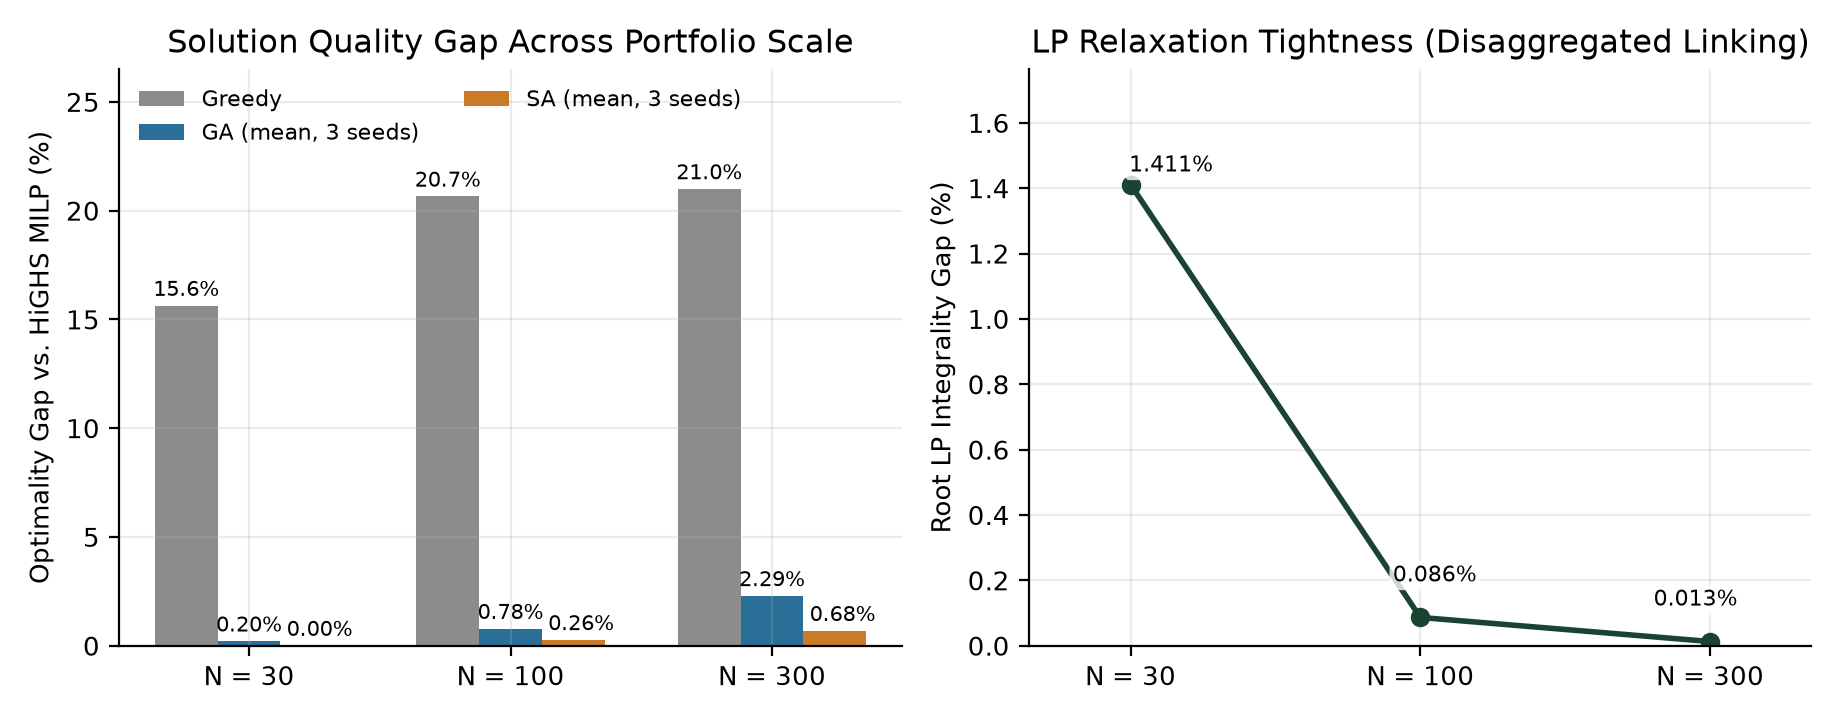
\includegraphics[width=0.86\textwidth]{fig_p1_scaling_gap.png}
\caption{Optimality gap scaling relative to HiGHS MILP (left) and root LP integrality gap collapse under disaggregated linking (right).}
\label{fig:gap}
\end{figure}

\begin{figure}[!ht]
\centering
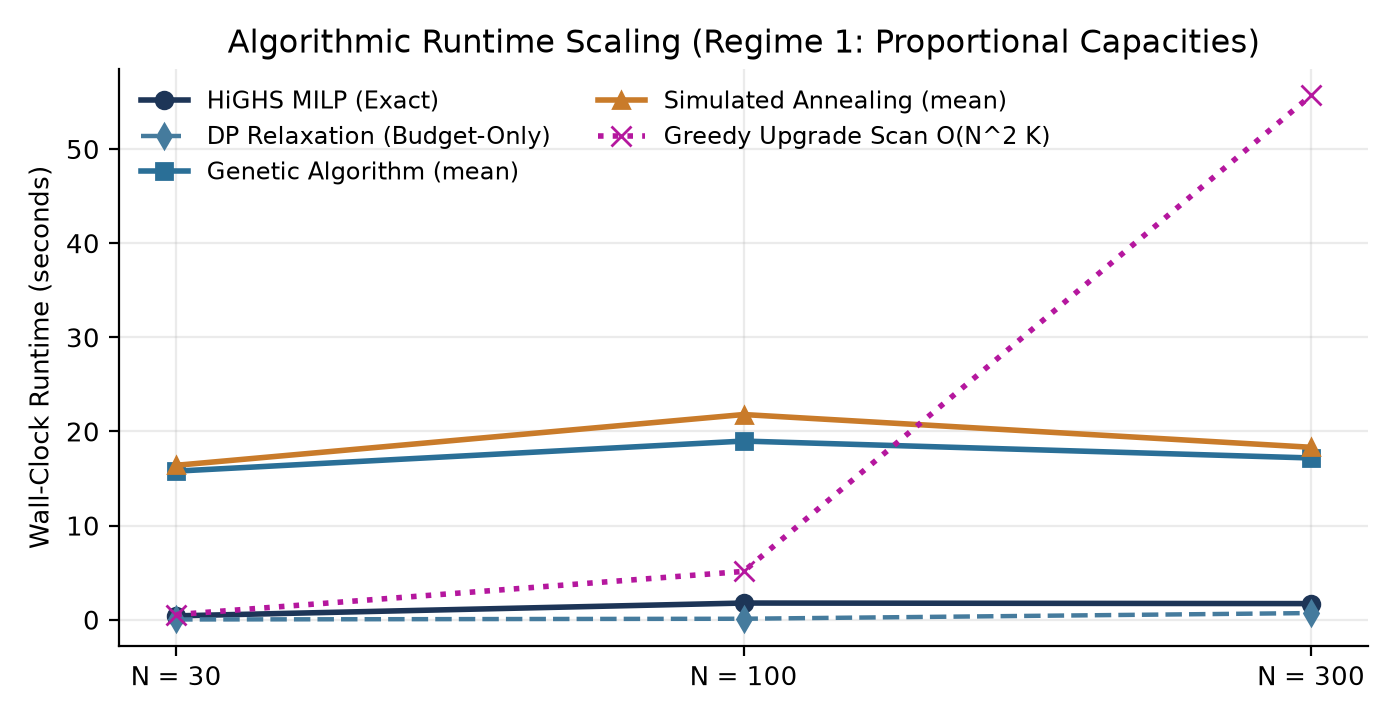
\includegraphics[width=0.72\textwidth]{fig_p1_scaling_time.png}
\caption{Wall-clock CPU runtime across portfolio scale ($N=30, 100, 300$, proportional capacity regime).}
\label{fig:time}
\end{figure}

\subsection{Bound Hierarchy, Custom B\&B, and SA Ablation}
\begin{itemize}
    \item \textbf{Dynamic Programming Upper Bounds:} Solving budget-only DP required $0.01$--$0.70\text{ s}$, yielding infeasible upper bounds \text{THB~}1,148,052 ($N=30$ main, 24 hard cases $>$ 10), \text{THB~}1,411,998 ($N=30$ B), \text{THB~}4,416,394 ($N=100$ prop), and \text{THB~}16,074,847 ($N=300$ prop, 222 hard cases $>$ 100). Across all runs, the strict bound hierarchy $Z_{\text{DP}} \ge \bar{Z}_{\text{LP}} \ge Z^* \ge Z_{\text{SA}} \ge Z_{\text{GA}} \gg Z_{\text{Greedy}}$ holds without exception.
    \item \textbf{Custom Branch-and-Bound:} On \texttt{N30\_unseenB}, custom B\&B proved optimality in \texttt{1,697} nodes ($848$ pruned, \texttt{11.80 s}). On \texttt{N30\_main}, B\&B located exact $Z^* = \text{THB~}1{,}099{,}661.34$ within a \texttt{10,000}-node budget ($1{,}396$ pruned, \texttt{141.0 s}, heap still open due to tied LP relaxations; the \texttt{20,000}-node log in \texttt{results\_N30.json} closed at \texttt{6,267} nodes). On \texttt{N100\_prop}, a \texttt{1,000}-node budget (\texttt{37.43 s}) remained stuck at the Greedy incumbent ($20.65\%$ gap).
    \item \textbf{SA Initial-Temperature Ablation (\texttt{N30\_main}):} Across 3 seeds with $T_0 = 20{,}000$, all runs froze prematurely at \text{THB~}944,293.22 ($14.13\%$ gap, $y=0$, zero legal cases), whereas $T_0 = 10^6$ hit $Z^*$ on $3/3$ seeds ($0.000\%$ gap). Figure~\ref{fig:conv} shows convergence trajectories.
    \item \textbf{Statistical Test:} Across all 18 paired stochastic runs (6 instances $\times$ 3 seeds), SA achieved an overall mean gap of $0.720\%$ vs. GA's $1.816\%$ (two-sided Wilcoxon signed-rank test, $W = 1.0$, $p = 0.00035$).
\end{itemize}

\begin{figure}[!ht]
\centering
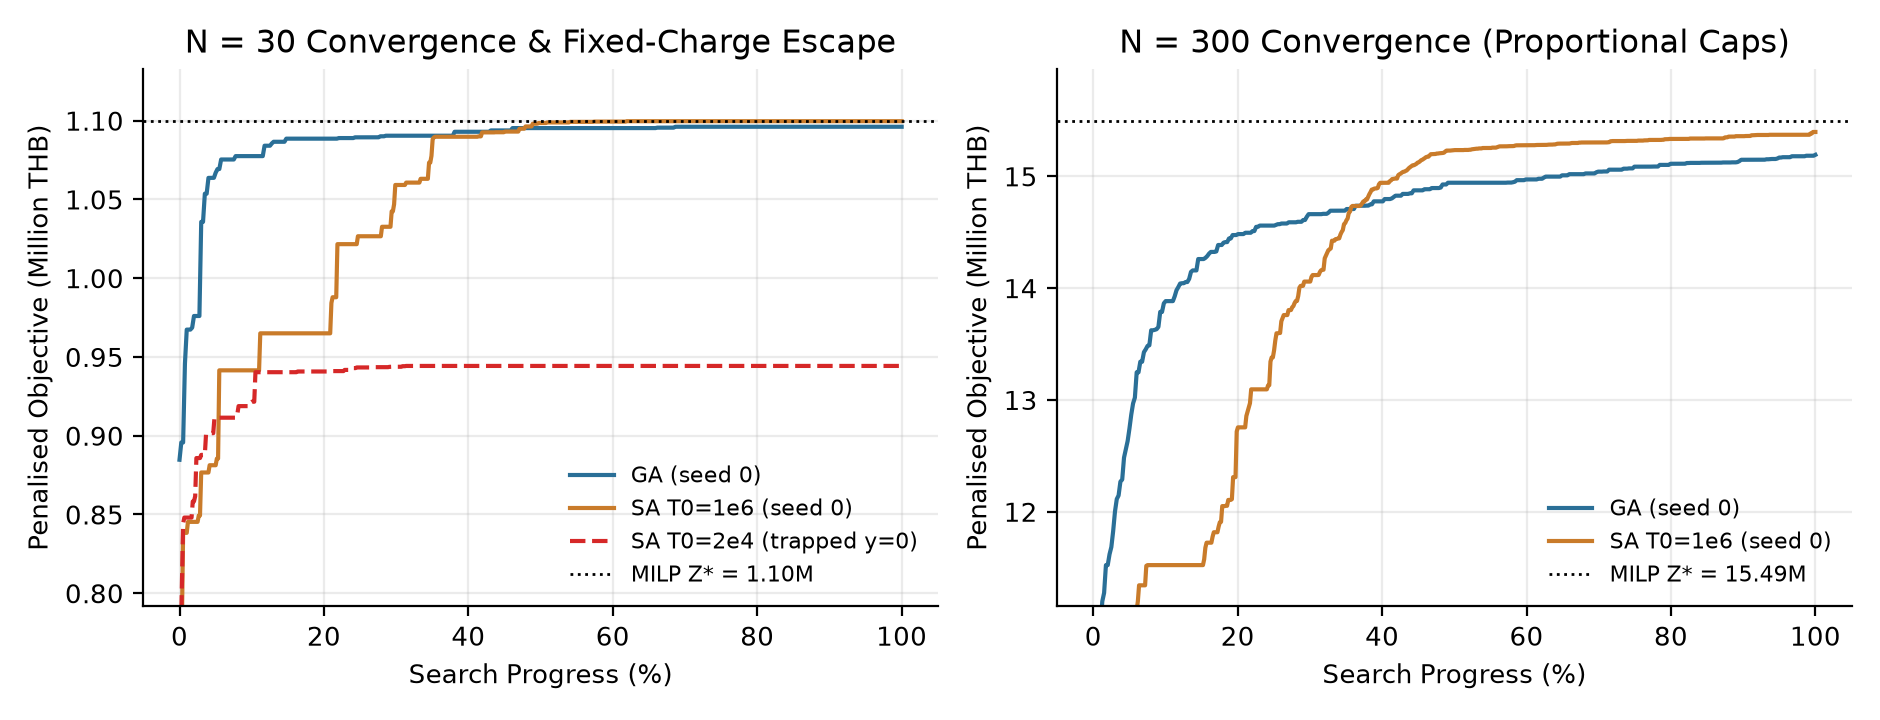
\includegraphics[width=0.86\textwidth]{fig_p1_convergence_ablation.png}
\caption{Search convergence on $N=30$ showing SA retainer-barrier trapping at $T_0=2\times 10^4$ (left) and $N=300$ scaling behavior (right).}
\label{fig:conv}
\end{figure}

\subsection{Optimal Strategy Allocation and Sensitivity Analysis}
Table~\ref{tab:sensitivity} details resource utilization, LP shadow prices, and strategy mixes. Figure~\ref{fig:mix} compares channel proportions across regimes.

\begin{table}[!ht]
\centering
\caption{Optimal allocation mix, cost, and LP shadow prices across scales and capacity regimes.}
\label{tab:sensitivity}
\scriptsize
\begin{tabular*}{\textwidth}{@{\extracolsep{\fill}}l r l r r r r@{}}
\toprule
\textbf{Instance} & \textbf{Cost / Cap (THB)} & \textbf{Mix (\texttt{0/1/2/3/4/5})} & \textbf{$\partial Z / \partial B_{\max}$} & \textbf{$\partial Z / \partial H$} & \textbf{$\partial Z / \partial V$} & \textbf{$\partial Z / \partial M$} \\
\midrule
\texttt{N30\_main} & 147,575 / 150,000 & \texttt{0 / 1 / 14 / 5 / 5 / 5} & THB~1.28 / THB~1 & THB~0.00 / h & THB~7,687 / visit & THB~7,113 / acct \\
\texttt{N30\_unseenB} & 149,941 / 150,000 & \texttt{0 / 1 / 14 / 5 / 6 / 4} & THB~1.51 / THB~1 & THB~0.00 / h & THB~7,915 / visit & THB~6,818 / acct \\
\texttt{N100\_prop} & 499,890 / 500,000 & \texttt{1 / 4 / 45 / 17 / 13 / 20} & THB~1.51 / THB~1 & THB~0.00 / h & THB~6,944 / visit & THB~6,817 / acct \\
\texttt{N300\_prop} & 1,499,998 / 1,500,000 & \texttt{7 / 14 / 129 / 50 / 40 / 60} & THB~1.78 / THB~1 & THB~0.00 / h & THB~9,041 / visit & THB~8,207 / acct \\
\texttt{N100\_frozen} & 148,628 / 150,000 & \texttt{7 / 62 / 16 / 5 / 6 / 4} & THB~2.08 / THB~1 & THB~16,937 / h & THB~32,859 / visit & THB~28,894 / acct \\
\texttt{N300\_frozen} & 149,988 / 150,000 & \texttt{37 / 232 / 16 / 5 / 7 / 3} & THB~2.75 / THB~1 & THB~42,910 / h & THB~71,653 / visit & THB~65,174 / acct \\
\bottomrule
\end{tabular*}
\end{table}

\begin{figure}[!ht]
\centering
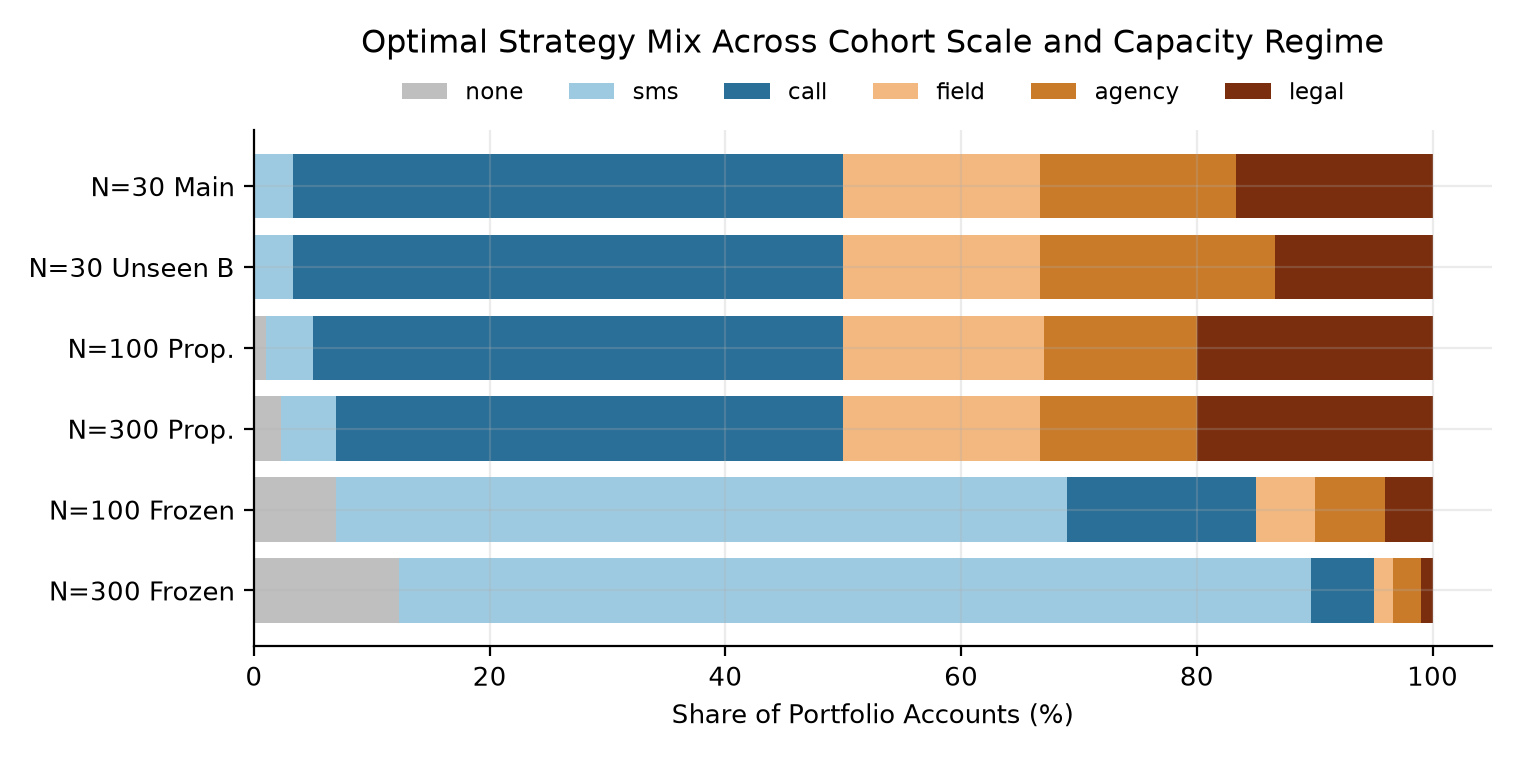
\includegraphics[width=0.75\textwidth]{fig_p1_strategy_mix_scales.png}
\caption{Optimal allocation share by channel across cohorts and capacity regimes.}
\label{fig:mix}
\end{figure}

\section{Result Discussion and Verification}

\subsection{Operational Interpretation of Empirical Findings}
\begin{enumerate}
    \item \textbf{Why Greedy Fails ($14.4\%\text{--}21.0\%$ Gap):} Evaluating single-account marginal ratios ($\Delta Z / \Delta \text{cost}$) never triggers litigation ($y=0$), because assigning legal action to one borrower incurs the full $\text{THB~}40{,}000$ retainer fee and violates $L=3$. Consequently, Greedy diverts high-balance accounts to external agencies ($25\%$ commission), spending only $\text{THB~}18{,}925$ on \texttt{N30\_main} and leaving $\text{THB~}171{,}881$ of net value uncaptured. Moreover, its nested upgrade loop scales as $\mathcal{O}(N^2 K)$, taking \texttt{55.70 s} at $N=300$---nearly $3\times$ slower than SA or GA.
    \item \textbf{Shadow Prices Reveal Bottlenecks:} Under proportional scaling, call-center hours carry zero shadow price ($10.5/12\text{ h}$ used at $N=30$, $96.75/120\text{ h}$ at $N=300$), meaning overtime hiring adds zero value. Conversely, budget, field visits ($\text{THB~}7.7\text{k--}9.0\text{k}$ per visit vs. $\sim \text{THB~}2.5\text{k}$ field cost), and conduct cap $M$ bind tightly. Under frozen staffing (\texttt{N300\_frozen}), the optimizer shifts $77.3\%$ of accounts (\texttt{232/300}) to low-cost SMS/LINE, yet still allocates the exact minimum $L=3$ litigation cases while call-hour marginal value rises to $\text{THB~}42{,}910/\text{h}$.
    \item \textbf{Retainer Invariance Confirmed:} Treating $F$ and $L$ as fixed contract constants independent of $N$ preserves model validity. An exploratory test erroneously scaling $L \propto N/30$ ($L=30$ at $N=300$) erected a $3\text{M}$ penalty wall that locked SA in the $y=0$ basin ($19.86\%$ gap), whereas fixed $L=3$ yielded a $0.683\%$ SA mean gap.
\end{enumerate}

\subsection{Exact vs. Meta-Heuristic Trade-Offs (Verification)}
All MILP and stochastic incumbents passed exact constraint verification (\texttt{violation == 0.0} across all 36 GA/SA runs and 6 MILP solutions). Comparing algorithms yields an honest methodological trade-off:
\begin{itemize}
    \item \textbf{Where Exact MILP Wins:} Because the formulation is linear and disaggregated linking ($x_{i,5} \le y$) keeps the continuous polytope tight---shrinking the root LP gap from $1.411\%$ ($N=30$) to $0.013\%$ ($N=300$, only $4$ fractional variables out of $1{,}625$)---compiled C++ HiGHS solves all instances in $0.40$--$2.01\text{ s}$ with a $0\%$ optimality certificate. Meta-heuristics do not outperform HiGHS in runtime or precision on linear problems of this size.
    \item \textbf{Why SA Outperforms GA ($p = 0.00035$):} At $N=300$, uniform crossover splices half of each parent's $300$-gene assignment vector simultaneously, disrupting delicately balanced resource feasibility and widening GA's gap to $2.287\%$ ($\text{SD} = 71{,}639$). Simulated Annealing executes local 1-gene flips ($70\%$) and pairwise swaps ($30\%$), maintaining near-saturated constraint efficiency ($0.683\%$ gap at $N=300$) while escaping the initial retainer barrier via $T_0 = 10^6$.
    \item \textbf{Role of Meta-Heuristics Relative to Custom B\&B:} Our pure-Python Branch-and-Bound solver already stalls within $1{,}000$ nodes on $N=100$, whereas SA and GA scale near-linearly in evaluation cost ($16$--$29\text{ s}$) with guaranteed feasibility. More practically, exact MILP requires linear separability; real-world non-linear multi-touch response saturation or black-box uplift predictors break linear formulations, making an integer-vector SA/GA engine necessary once linear assumptions are relaxed in Phase~II.
\end{itemize}

{\small
\begin{thebibliography}{99}
\setlength{\itemsep}{0.5pt}
\setlength{\parskip}{0pt}
\bibitem{taha2017} H.~A. Taha, \emph{Operations Research: An Introduction}, 10th~ed. Pearson, 2017.
\bibitem{land1960} A.~H. Land and A.~G. Doig, ``An automatic method of solving discrete programming problems,'' \emph{Econometrica}, vol.~28, no.~3, pp. 497--520, 1960.
\bibitem{highs2018} Q.~Huangfu and J.~A.~J. Hall, ``Parallelizing the dual revised simplex method,'' \emph{Math. Program. Comput.}, vol.~10, no.~1, pp. 119--142, 2018.
\bibitem{sinha1979} P.~Sinha and A.~A. Zoltners, ``The multiple-choice knapsack problem,'' \emph{Oper. Res.}, vol.~27, no.~3, pp. 503--515, 1979.
\bibitem{kellerer2004} H.~Kellerer, U.~Pferschy, and D.~Pisinger, \emph{Knapsack Problems}. Springer, 2004.
\bibitem{goldberg1989} D.~E. Goldberg, \emph{Genetic Algorithms in Search, Optimization, and Machine Learning}. Addison-Wesley, 1989.
\bibitem{kirkpatrick1983} S.~Kirkpatrick, C.~D. Gelatt, and M.~P. Vecchi, ``Optimization by simulated annealing,'' \emph{Science}, vol.~220, no.~4598, pp. 671--680, 1983.
\bibitem{haimes1971} Y.~Y. Haimes, L.~S. Lasdon, and D.~A. Wismer, ``On a bicriterion formulation of integrated system identification and optimization,'' \emph{IEEE Trans. Syst., Man, Cybern.}, vol.~SMC-1, no.~3, pp. 296--297, 1971.
\bibitem{scipy2020} P.~Virtanen \emph{et~al.}, ``SciPy 1.0: Fundamental algorithms for scientific computing in Python,'' \emph{Nat. Methods}, vol.~17, pp. 261--272, 2020.
\bibitem{sklearn2011} F.~Pedregosa \emph{et~al.}, ``Scikit-learn: Machine learning in Python,'' \emph{J. Mach. Learn. Res.}, vol.~12, pp. 2825--2830, 2011.
\bibitem{lendingclub} Kaggle, ``Lending Club loan data: Financial recovery and charge-off records,'' \url{https://www.kaggle.com/datasets/adarshsng/lending-club-loan-data-csv}, 2019.
\bibitem{thaidebtact} Kingdom of Thailand, ``Debt Collection Act B.E. 2558 (2015),'' \emph{Royal Thai Government Gazette}, vol.~132, Part~16~A, 2015.
\end{thebibliography}
}

\end{document}
